% !TeX root = Synopse.tex

\documentclass[12pt]{article}
\usepackage{lingmacros}
\usepackage{tree-dvips}
\usepackage[utf8]{inputenc}
\usepackage{fancyhdr}
\usepackage{listings}
\usepackage{subfig}
\usepackage{xcolor}
\usepackage{geometry}
\geometry{
a4paper,
total={170mm,257mm},
left=15mm,
top=20mm,
}
\usepackage{graphicx}
\usepackage{wrapfig}
\usepackage{amsmath}
\usepackage{hyperref}
\definecolor{link}{rgb}{0,0,215}
\hypersetup{
    colorlinks=true,
    linkcolor=link,
    filecolor=link,      
    urlcolor=link,
    pdfpagemode=FullScreen,
}

\graphicspath{ {./img} }

\definecolor{comment}{rgb}{0,0.45,0}
\definecolor{codegray}{rgb}{0.5,0.5,0.5}
\definecolor{codepurple}{rgb}{0.58,0,0.82}
\definecolor{backcolour}{rgb}{0.95,0.95,0.92}
\lstdefinestyle{CodeStyle}{
    backgroundcolor=\color{backcolour},   
    commentstyle=\color{comment},
    keywordstyle=\color{magenta},
    numberstyle=\tiny\color{codegray},
    stringstyle=\color{codepurple},
    basicstyle=\ttfamily\footnotesize,
    breakatwhitespace=false,         
    breaklines=true,                 
    captionpos=b,                    
    keepspaces=true,                 
    numbers=left,                    
    numbersep=5pt,                  
    showspaces=false,                
    showstringspaces=false,
    showtabs=false,                  
    tabsize=2
}
\lstset{style=CodeStyle}
\lstdefinelanguage{JavaScript}{
  keywords={typeof, new, true, false, catch, function, return, null, catch, switch, var, if, in, while, do, else, case, break},
  keywordstyle=\color{purple}\bfseries,
  ndkeywords={class, export, const, var, let, boolean, throw, implements, import, this, !!, !=, ===, ;},
  ndkeywordstyle=\color{blue}\bfseries,
  identifierstyle=\color{black},
  sensitive=false,
  comment=[l]{//},
  morecomment=[s]{/*}{*/},
  commentstyle=\color{comment}\ttfamily,
  stringstyle=\color{orange}\ttfamily,
  morestring=[b]',
  morestring=[b]"
}

%%%%%%% Document begin %%%%%%%%%%%
\begin{document}
\title{A* Algoritme}
\author{Johannes Jørgensen\\ S3o}
\date{2023 Febuar}
\maketitle
\textit{Projektets godkendelse og gennemgang af forløb.}\\
Mit projekt (som er Pathfinding algoritmer) har jeg lavet lidt ændringer i mit gamle projekt, så den gamle kode er klar til at blive bygget videre på. Jeg vil gerne nå at implementere et vægtsystem i mit projekt, så min algoritmer kan blive lidt mere realistisk. Dette er til så min pathfinder skal kunne vurdere hvilken vej er nemmest og hurtigst vej fra A til B. Jeg er ikke begyndt endnu at implementere en ny algoritme (Jeg tænker A-star), da jeg først vil være klar med min gamle kode, samt have SOP overstået.  
Næste gang skal jeg også have lavet noget research inden for vægtet pathfinding, som jeg tænker er mit næste skridt i projektet. 
Efter det skal jeg implementere det og derefter gå videre med at implementere A-star algoritmen (måske nogle andre hvis jeg har tid)
Hvis jeg har meget tid til overs kan jeg gøre det visuelle mere lækkert at se på. \\
\textit{Se evt. hele programmet på:} \href{https://github.com/johannes67890/Pathfinding.git}{Github.com/johannes67890/Pathfinding} 
\tableofcontents
\pagebreak

%% Introduktion
\section{Introduktion}
Når du indtaster en destination ind på Google Maps på din telefon, hvordan finder Google Maps så den hurtigste vej? Kompleksiteten som Google Maps har for at finde den hurtigste vej er umådelig stor, men en af elementerne som Google Maps bruger er Pathfinding Algoritmer. Formålet ved pathfinding algoritmer er at finde den korteste vej fra $a$ til $b$.
Jeg har i mit projekt opbygget et program som fremviser hvordan forskellige pathfinding algoritmer virker. Denne fremvisning er en visuel fremstilling af hvordan algoritmen påvirker et gitter miljø med forhindringer (vægge). Dette projekt bygger videre på mit tidligere projekt som jeg har lavet i 2.g hvor jeg havde en visuel fremstilling af Dijkstra’s algoritme. Men jeg har nu med et nyt design implementeret Astar (A*) algoritmen, som jeg vil have fokus på.

%% Teori
\section{Problemformulering}
Hvordan kan man med brug af Astar algoritme bruge ”Heuristics” til at finde den korteste vej fra $a$ til $b$ mest effektivt?
\section{Programbeskrivelse}
Mit program er en visuel fremvisning over hvordan pathfinding algoritmer fungerer og ”bevæger” sig i forhold til miljøet. Programmet er en webapplikation opbygget med et gitter af nogle celler, en ”Start” knap og forskellige indstillinger. 
Gitteren er hovedkomponentet i programmet, der er gitteret som er miljøet som pathfinding algoritmerne bevæger sig i. Miljøet kan brugeren selv ændre, med at placere og fjerne vægge som pathfinding algoritmerne ikke kan gå igennem. Dette gør det muligt for at brugeren kan eksperimentere med de forskellige algoritmer, samt udforske hvad algoritmerne vil gøre i forskellige situationer. Brugeren kan ændre forskellige indstiller som vil have effekt på hvordan algoritmen opføre sig. Disse forskellige indstillinger inkluderer størrelsen af gitteret (samt antallet af celler i gitteret), hastigheden på algoritmens køretid, Hvilken algoritme som skal køres og muligheden for at sætte tilfældige væge. 

\section{Teori}
A* (udtalt ”A-star”) eller Dijkstra er begge en algoritme i ”Pathfinding”, som er en computer applikation af den korteste vej mellem to punkter. Når der er tale om Pathfinding algoritmer og grafteori, skal vi først gennemgå forskellige relevante emner for at kunne bedre forstå problemet som pathfinding algoritmer løser. Her er det relevant at snakke om data-trees, Breadth-First Search (BFS) og Depth-first search (DFS). 
\subsection{Data-trees}
Data-trees inde for grafteori er en populær måde at bruge som en abstrakt form for data type, som repræsenterer et hierarkisk data-tree med forbundet ”celler” (”nodes” bliver brugt i samme sammenhæng). Hver cell er forbundet til en ”parent” cell, bortset fra start cellen eller roden af data-treet, som ingen parent cell har. Disse begrænsninger betyder, at der ikke er nogen cyklusser og at hvert ”child” cell kan behandles som roden af sit eget ”subtree” (et indsnævret  mængde af celler i et større data-tree). Disse elementer gør at rekursion kan bruges som en brugbar teknik inden for data-trees.\\
Der er flere forskellige metoder som bruges for at finde den korteste vej i et stort netværk af punkter og parameter.\footnote{\href{https://www.geeksforgeeks.org/introduction-to-tree-data-structure-and-algorithm-tutorials/}{Introduction to Tree - Data Structure and Algorithm Tutorials}} De to mest velkendte algoritmer er Breadth-First Search (BFS) og Depth-first search (DFS). 
Breadth-First Search algoritme søger de tætteste naboer før algoritmen går videre til det næste led af data celles i data-tree. Dette gør algoritmen uden forhold til nogle parametre eller ekstra viden om netværket den søger igennem. Depth-first search gør det omvendte af BFS, her søger DFS algoritmen først gennem en enkel gren før den gør tilbage til start cellen og gør det samme med en anden gren i data-tree. 
\begin{figure}[ht]%
  \centering
  \subfloat[\centering Struktur for et data-tree]{{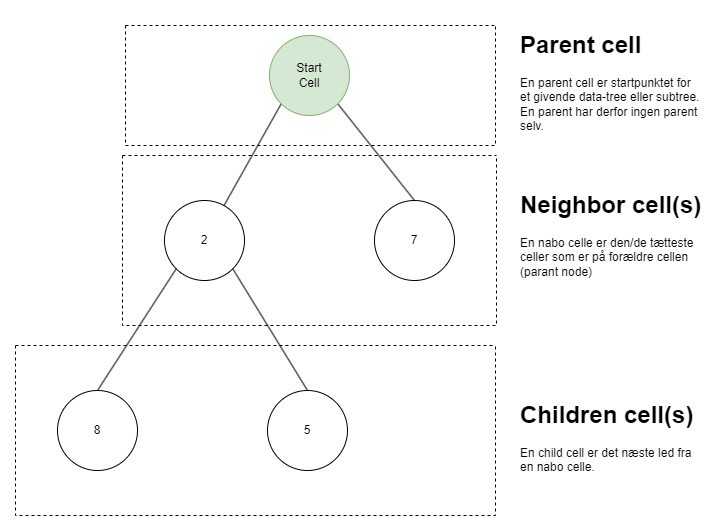
\includegraphics[width=0.85\textwidth]{../datatree.png} }}%
  \label{fig:datatree}%
\end{figure}
\subsection{Dijkstra’s algoritme}
Dijkstra’s algoritme er en variation af Breadth-First Search, men hvor Dijkstra’s algoritme gør brug af en prioriterings kø, som afgør hvilken nabo Dijkstra skal søge igennem først. 
Dijkstra starter med at angive en arbitrær afstandsværdi til alle celler i netværket: start cellen får afstandsværdien 0, hvor alle andre får afstandsværdien Infinity. 
Vores prioteringskø holder vi øje med alle undersøgte celler. For den nuværende celle, bliver alle naboer som ikke er undersøgt med (afstanden til nuværende celle) + (afstanden fra nuværende celle til naboen). Hvis denne afstandsværdi er mindre end den forrige arbitrær afstandsværdi, bliver den nye afstand værdi kun relevant. Når vi er færdige med at undersøge afstandsværdien for alle naboer, markere vi den nuværende celle som undersøgt.\footnote{\href{https://en.wikipedia.org/wiki/Dijkstra%27s_algorithm}{Dijkstra's algorithm}}  

\subsection{A* algoritme}
A-star algoritmen er en videreudvikling af Dijkstra’s algoritme. Denne forlængelse er ved brug af målrettet heuristik, 
som gør det muligt for A-star at vide hvilke ruter som skal søges igennem først. 
Heuristik gør derfor A-star til en informeret søgealgoritme, eller en best-first search algoritme. 
Ved hver iteration af A-stars loop, skal algoritmen tag stilling til hvilken rute som skal søges. Dette gøres den baseret på omkostningerne af den rute, samt rutes estimeret omkostning som skal til for at bruge den rute hele vejen til slut.\footnote{\href{http://theory.stanford.edu/~amitp/GameProgramming/AStarComparison.html}{Introduction to A* (Standford)}} A-star brugere tre forskellige værdier til at beslutte dette: 
(hvor $n$ er den næste celle på den på givende rute)\\
\[g(n)\]
$g(n)$  er omkostningerne af ruten fra start til $n$.
\[h(n)\] 
$h(n)$ er den heuristiske værdi som estimerer omkostningerne af den billigste rute fra celle n til slut. 
Der er flere forskellige måder at beregne h værdien, enten beregne det præcise værdi for $h$ (dette kan kræve meget tid) eller en estimeret værdi for $h$ som tag mindre tid. En af disse måder kunne være med \textit{Manhattan Distance.} 
Manhattan Distance er summen af absolutte værdier af forskellen af henholdsvis X- og Y-koordinater mellem start og slut cellen. 
\begin{lstlisting}[language=JavaScript, caption=Manhattan Distance\label{code:Manhattan}]
  h = abs(current_cell.x - goal.x) + 
  abs(current_cell.y - goal.y)
\end{lstlisting}
\begin{figure}[ht]\label{fig:Manhattan}
  \centering
  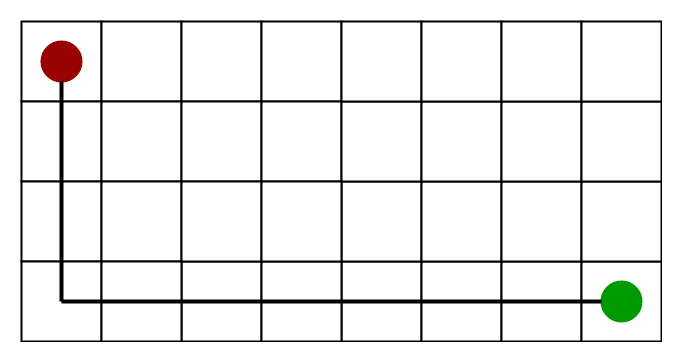
\includegraphics[width=0.50\textwidth]{../manhattan.png}
  \caption{Manhattan Distance Heuristics, med forskellen mellem x og y-koordinaterne (Evt. antag at rød plet er start cellen og grøn er slut cellen)}
\end{figure}
Efter beregningerne af $g(n)$ og $h(n)$, beregner vi den tredje værdi $f(n)$, 
som repræsenterer vores nuværende bedste gæt til den billigste vej fra start til slut:
\[f(n)= g(n) + h(n)\]
\section{Funktionalitet}
Det er vigtigt at når brugeren åbnet programmet, at de ikke er i tvivl om hvad der foregår. For at kunne opnå en høj funktionalitet opstiller jeg nogle krav. Dette inkluderer hvordan man køre algoritmen, vælger hastighed, gitter størrelse og sætte vægge. Samtidig skal det være intuitivt at se hvad der forgår, selvom man ikke forstår pathfinding. 
\begin{itemize}
  \item Brugeren skal kunne klikke på enkle punkter på gitteret for at kunne tilføje eller fjerne en væg, samt kunne nemt forstå at en væg er blevet fjernet eller tilføjet. 
  \item Det skal samtidig være simpelt at kunne ændre på nogle indstillinger for f.eks. hvor hurtig algoritmen køre eller hvor stort et gitter man vil bruge. 
  \item Når brugeren kører programmet, skal det være intuitivt at kunne forstå hvordan algoritmen fungere og hvilken vej som er den korteste fra $a$ til $b$.
\end{itemize}
\newpage
\section{Brugergrænseflade}
Når et it-produkt bliver produceret og designet, er det vigtigt at brugeren af programmet kan anvende det uden irritation eller følelsen af utilstrækkelighed. Man designer derfor en brugergrænseflade som fokuserer på at gøre it-produktet tilfredsstillende for brugeren.
En brugergrænseflade er en form for bindeled mellem en bruger og et it-produkt eller system. Brugergrænsefladen modtager forskellige typer af inputs fra bruger, såsom klik med musen eller via tastaturet osv. Det input giver derefter et output og måske en form for feedback til brugeren, efter brugeren har interageret med it-produktet. 
\begin{table}[ht]
  \centering
  {\renewcommand{\arraystretch}{2.5} %<- modify value to suit your needs
  \begin{tabular}{ |c|c| }
   \hline
   \textbf{Input fra brugeren} & \textbf{Output} \\ 
   \hline
   Klik på celle i gitter & \shortstack{Tilføj eller fjern væg i forhold \\ til om der allerede er en væg eller ej.} \\
   \hline
   ’Drag’ skyder under ”Animation Speed” & \shortstack{Ændre hastigheden for \\ animationen for algoritmen i ms.} \\
   \hline
   Klik på ”Start” knappen & Starter programmet med valgt algoritme. \\
   \hline
   \shortstack{Klik på en af ”Cell Size” knapperne \\(Big, Default, Small)} & Ændre Størrelsen på cellerne i gitteret. \\
   \hline
   \shortstack{Klik på en af algoritmeknapperne \\ (Dijkstra eller Astar)} & \shortstack{Ændre valget algoritme som bliver \\kørt når ”Start” knappen bliver trykket.} \\
   \hline
   Klik på ”random walls” knappen & \shortstack{Placere tilfældige væge i gitteret \\ som algoritmerne ikke må gå igennem.} \\
   \hline
  \end{tabular}}
\end{table}
\section{Modeller og Diagrammer}
For at få en bedre forståelse for et givende it-system, kan diverse modeller og diagrammer være med til at give overblik. 
Dette kan ske for både hvordan enkle algoritmer fungere, hvordan klasser spiller sammen i programmet eller lignede. Når det kommer til Pathfinding algoritmer og et virsuelt program, 
er det brugbart at vide 
hvordan koden kobles sammen med diverse pathfinding algoritmer, samt hvordan DOM-elementerne (Et enkelt HTML element såsom <Div> eller <p>) på hjemmesiden bliver manipuleret. 
\newpage
\subsection{UML-diagram}
For at få en generelt overblik over et it-system, kan man bruge Unified Modeling Language (UML-diagrammer). Et UML-diagram kan beskrive strukturen og forløbet i et Objekt-orienteret it-system. Der er flere variationer til UML-diagrammer (Klasse diagram, Interaktionsdiagram osv.). 
Da mit program er opbygget i React (Et Javascript baseret frontend biblotek), er mit program opbygget af såkaldte ”Components” og ikke klasser. Derfor vil det ikke være muligt at lave et traditionelt klasse-diagram for et React system. Dette skyldes både at det er frontend baseret og DOM-elementer bliver manipuleret af ”states” (et objekt som indeholder data om React components og DOM-elementer). Jeg har derfor improviseret et UML-diagram som over styr på diverse state manipulationer på tværs af React components. 
Hele appen indeholder fire React componentes (”Cell”, ”Grid”, ”Header” og ”Algoritms”), som alle fælles kan implementere, manipulere eller brugere data fra de forskellige React ”Context's” (Et React som lader dig udsende data på tværs af flere React components ad gangen). Samtidig bruger hele appen to forskellige ”interfaces” (en selvbeskrev datatype) og konstanter som beskriver gitterstørrelsen og informationen for en enkel celle. Enkle React components har ”Child components”, private states og lignede, som hver er med til at manipulere med DOM-elementer. 
\begin{figure}[ht]\label{fig:UML}
  \centering
  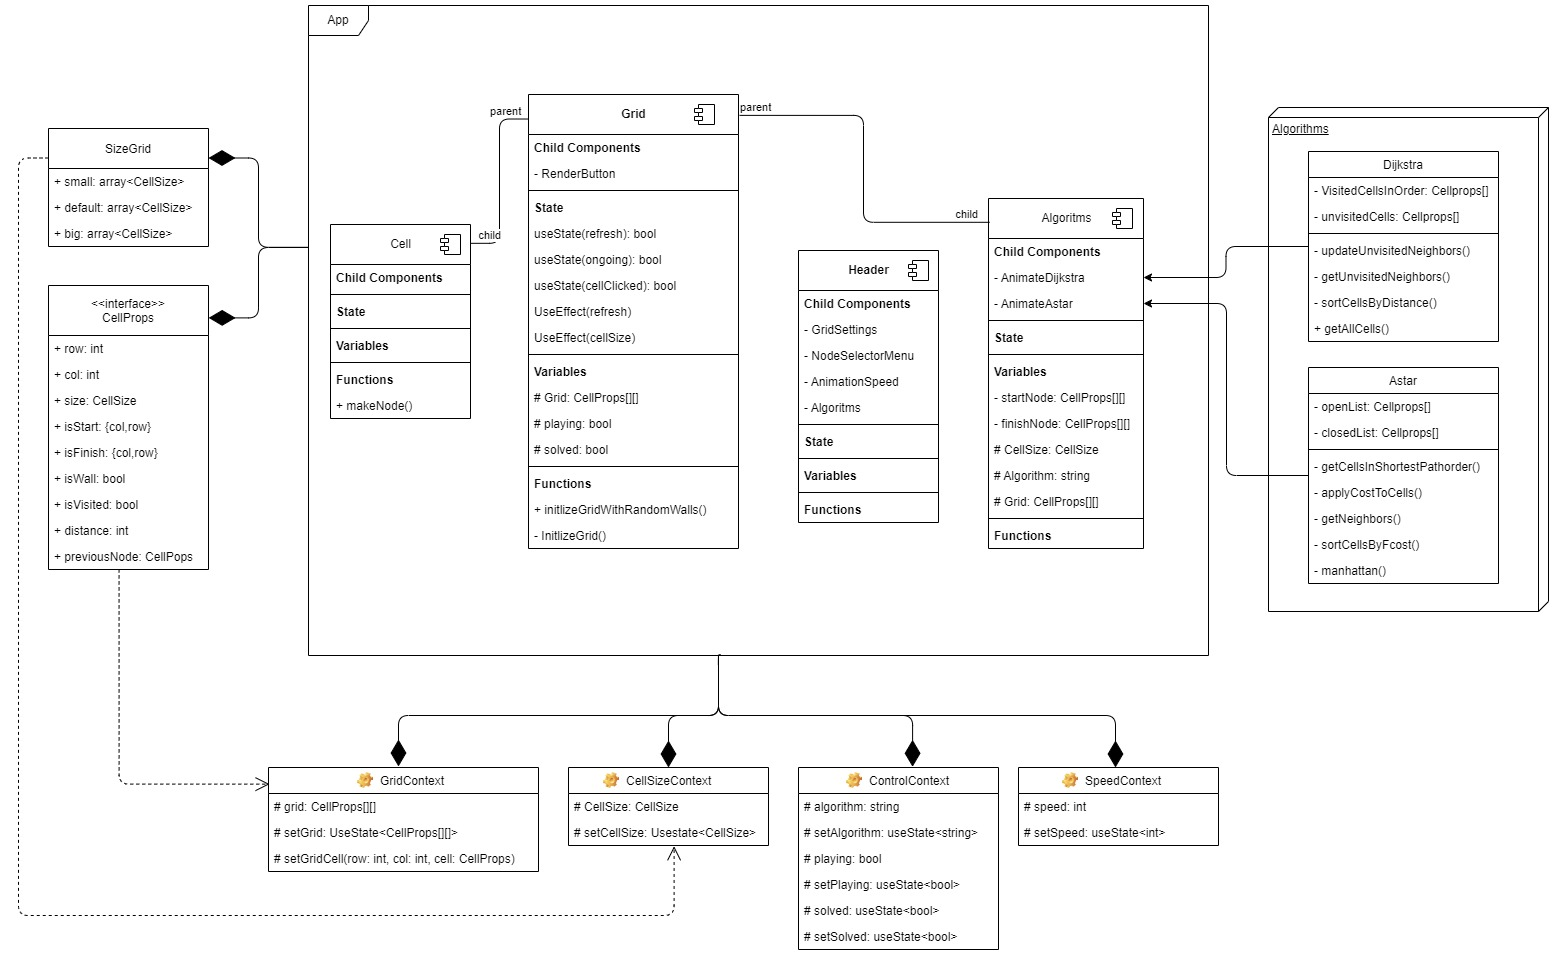
\includegraphics[width=1.1\textwidth]{../UML.jpg}
  \caption{UML-diagram for React components og states.}
\end{figure}

\newpage

\subsection{A* algoritme Pseudocode}
For at kunne skitsere hvordan en algoritme virker i praksis, kan vi gøre brug af pseudokode. Når vi bruger pseudokode som skitse, har det til formål at beskrive en enkel algoritme step-by-step som samtidig er let læselig for mennesker. Pseudokode bruger ikke direkte kodesprog, samt har heller ikke nogen fast syntaks for at undgå forvirring mellem forskellige kodesprog.\footnote{\href{https://en.wikipedia.org/wiki/A*_search_algorithm}{A-star Algorithm Pseudokode}}
\begin{lstlisting}[language=JavaScript, caption=Dijkstra’s Algorithm Pseudocode oversat til Dansk]
// A* finds a path from start to goal.
// h is the heuristic function. h(n) estimates the cost to reach goal from node n.
function A_Star(start, goal, h)
  // The set of discovered nodes that may need to be (re-)expanded.
  // Initially, only the start node is known.
  // This is usually implemented as a min-heap or priority queue rather than a hash-set.
  openSet := {start}

  // For node n, cameFrom[n] is the node immediately preceding it on the cheapest path from start
  // to n currently known.
  cameFrom := an empty map

  // For node n, gScore[n] is the cost of the cheapest path from start to n currently known.
  gScore := map with default value of Infinity
  gScore[start] := 0

  // For node n, fScore[n] := gScore[n] + h(n). fScore[n] represents our current best guess as to
  // how cheap a path could be from start to finish if it goes through n.
  fScore := map with default value of Infinity
  fScore[start] := h(start)

  while openSet is not empty
      // This operation can occur in O(Log(N)) time if openSet is a min-heap or a priority queue
      current := the node in openSet having the lowest fScore[] value
      if current = goal
          return reconstruct_path(cameFrom, current)

      openSet.Remove(current)
      for each neighbor of current
    // d(current,neighbor) is the weight of the edge from current to neighbor
    // tentative_gScore is the distance from start to the neighbor through current
          tentative_gScore := gScore[current] + d(current, neighbor)
          if tentative_gScore < gScore[neighbor]
    // This path to neighbor is better than any previous one. Record it!
              cameFrom[neighbor] := current
              gScore[neighbor] := tentative_gScore
              fScore[neighbor] := tentative_gScore + h(neighbor)
              if neighbor not in openSet
                  openSet.add(neighbor)

  // Open set is empty but goal was never reached
  return failure
\end{lstlisting}
\section{Udvalgt Kode}
Jeg har valgt at vise koden for A* algoritmen, da det er den algoritme jeg har brugt i mit program.
(Se kodeblock \ref{lst:A*}). Jeg vil fremvise hvordan jeg har implementeret en heuristisk funktion i mit program, samt hvordan jeg brugte samme funktion flere gange til nemmer implementering af algoritmen. \\
For at kunne finde vejen tilbage fra slut til start, gemmer jeg den forrige celle som jeg kan bruge til at ”back track” tilbage og dermed den korteste vej.

\begin{lstlisting}[language=JavaScript, caption=Find den korteste vej fra start til slut (A* algoritme)]
function getCellsInShortestPathOrderAstar(finishCell: CellProps) {
  const shortestPath: CellProps[] = [];
  let curr = finishCell;
  // Loop through all previous cells and add them to shortestPath
  while (curr.previousCell !== null) {
    shortestPath.push(curr);
    curr = curr.previousCell;
  }
  shortestPath.shift();
  return shortestPath.reverse();
}
\end{lstlisting}
Jeg har brugt Manhattan distance som heuristik funktion. 
Dette har jeg gjort da det var en nem måde at implementere i mit program. 
Mit gitter allerede var opsat i rækker og kolonner som kan repræsenteres som x- og y- retningen.
\begin{lstlisting}[language=JavaScript, caption=Heuristic function for A* algoritmen]
function manhattan(CurrCell: CellProps, finishCell: CellProps) {
  // Manhattan distance (Huristic)
  const h =
    Math.abs(CurrCell.row - finishCell.row) +
    Math.abs(CurrCell.col - finishCell.col);
  return h;
}
\end{lstlisting}
Samtidig har jeg brugt Manhattan distance som funktion til at uddeligere $f(n)$,$g(n)$ 
og $h(n)$ værdierne for individuelle celler i gitteret. f.eks. har blot brugt funktionen fra nuværende celle til startcellen til at give den nuværnde celle deres $g(n)$ værdi.  
\begin{lstlisting}[language=JavaScript, caption=Brug af Manhattan distance når cellerne skulle have deres $f(n)$ $g(n)$ og $h(n)$ værdier]
function applyCostToCells(
  grid: CellProps[][],
  startCell: CellProps,
  finishCell: CellProps
) {
  const newGrid = getAllCells(grid);
  for (const cell of newGrid) {
    if (cell.isWall) continue;
    if (cell.isStart) continue;
    if (cell.isFinish) continue;
    cell.cost.hCost = manhattan(cell, finishCell);
    cell.cost.gCost = manhattan(cell, startCell);
    cell.cost.fCost = cell.cost.gCost + cell.cost.hCost;
  }
}
\end{lstlisting}
\section{Resultater og Test}
For at opfylde de opstillet krav om at brugeren kan interagere med gitteret, algoritmens fungere og at den kan finde den korteste vej fra a til b. Kan vi lave forskellige test, såsom at samlingen min implantation af A-star med andre eller se om A-star gøre det bedre end Dijksta, som A-star skulle i teorien. Denne metode har jeg brugt til at teste hvorledes om min algoritme virker. \\
\begin{figure}[ht]
  \centering
  \subfloat[\centering Test af Dijksta]{{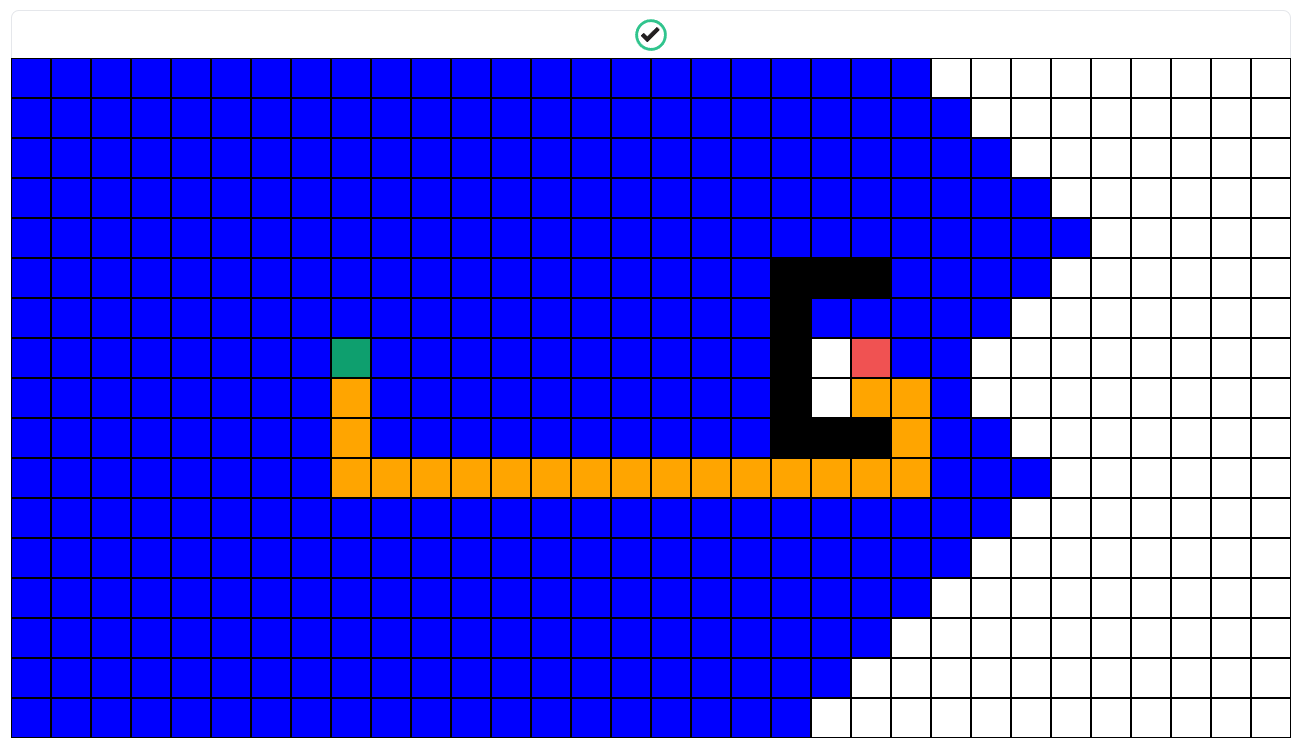
\includegraphics[width=9cm]{../Showcase_Dijkstra.PNG} }}%
  \subfloat[\centering Test af A* algoritmen]{{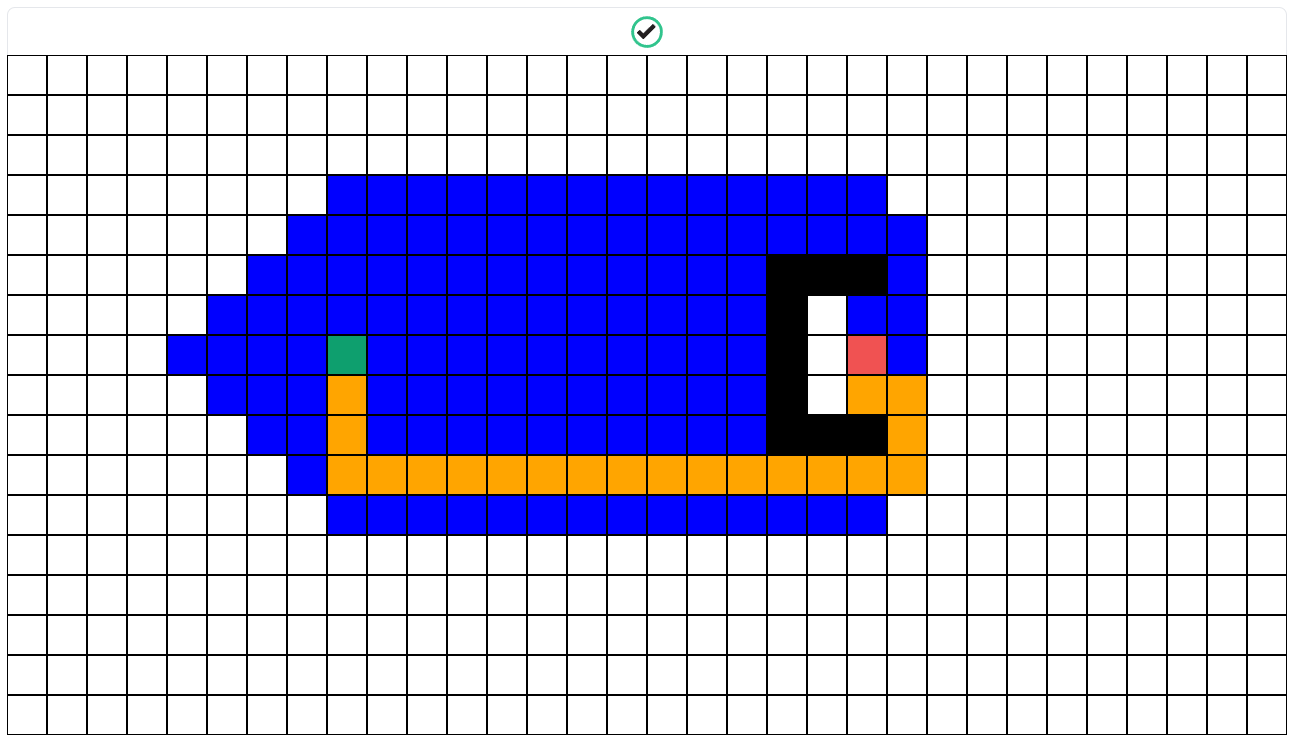
\includegraphics[width=9cm]{../Showcase_Astar.PNG} }}%
  \caption{Test af A* algoritmen VS. Dijksta algoritmen}\label{fig:testAlgortime}
\end{figure}
Der vises på figur \ref{fig:testAlgortime}, at der er stor forskel mellem mængden af undersøgte celler hos Dijksta, i forhold til A-star. Dette skulle det i teorien også være, da A-star ved hvor slut punktet nogenlunde er. Dermed er min test af min A-star algoritme godkendt. 
Vi kan teste om interaktionen med gitteret, animationshastighed osv. Fungere, med simpelt at prøve at se om det virker, samt om der er nogle bugs.
\begin{figure}[ht]
  \centering
  {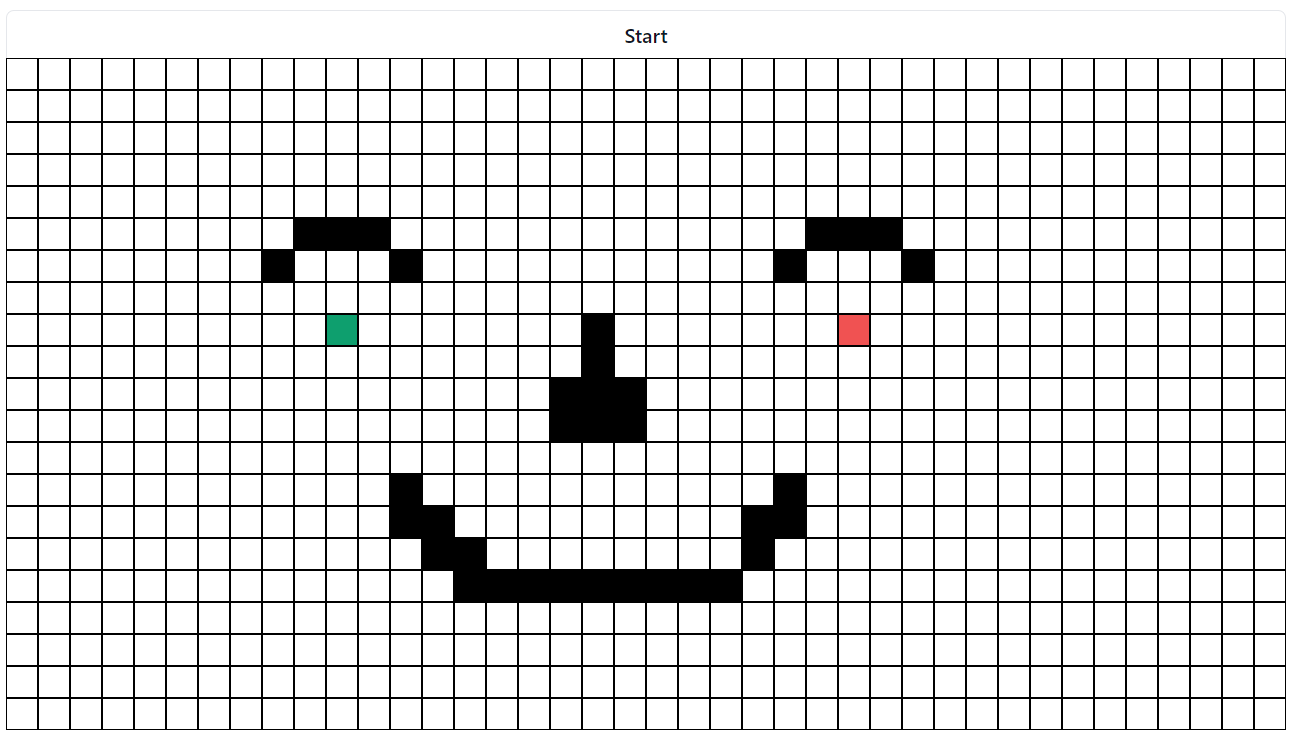
\includegraphics[width=9cm]{../AppPreview2.PNG} }%
  \caption{Test af interaktion med gitter}\label{fig:testInteraktion}
\end{figure}
\section{Konklusion}
Vi har undersøgt hvordan heuristik bliver brugt i pathfinding algorithmer som A-star, til at finde den hurtigste vej fra $a$ til $b$. Dette har vi gjort med både at se hvordan grafteorien fungere inden for pathfinding, men samtidig implementeret A-star og Dijkstra i et praksiseksempel på hvordan algoritmerne hver og sær bevæger sig. Vi kunne også konkludere at brug af heuristik kunne øge algoritmens ydeevne drastisk, med blot lidt information. Så næste gang Næste gang vi åbner Google Maps for at finde den hurtigste vej til den nærmeste Macdonalds, så har vi nu fået et lille indblik i hvordan Google Maps fungere for at finde den hurtigste vejen for os. 
\newpage
\section*{Bilag}
\begin{lstlisting}[language=JavaScript, caption=Udvalgt kode af A* algoritmen, label={lst:A*}]
  function astar( grid: CellProps[][], startCell: CellProps, finishCell: CellProps) {
    applyCostToCells(grid, startCell, finishCell); // Apply cost to all cells
    const openList: CellProps[] = []; // List of cells to be evaluated
    const closedList: CellProps[] = []; // List of cells already evaluated
    startCell.cost.gCost = 0;
    startCell.cost.hCost = manhattan(startCell, finishCell);
    startCell.cost.fCost = startCell.cost.gCost + startCell.cost.hCost;
    openList.push(startCell); // Add startCell to openList
  
    while (!!openList.length) {
      sortCellsByFcost(openList); // Sort openList by fCost (lowest to highest)
  
      // Find lowest fCost 
      let lowestIndex = 0;
      for (let i = 0; i < openList.length; i++) {
        if (openList[i].cost.fCost < openList[lowestIndex].cost.fCost) {
          lowestIndex = i;
        }
      }
      let current = openList[lowestIndex]; // Set current to lowest fCost
    
      if (current.isFinish) {
        // If current is finishCell, return closedList
        closedList.shift();
        return closedList;
      }
  
      openList.splice(lowestIndex, 1);
      closedList.push(current);
  
      let neighbors: CellProps[] = getNeighbors(current, grid);
      for (let i = 0; i < neighbors.length; i++) {
        let neighbor = neighbors[i];
        if (!closedList.includes(neighbor) && !neighbor.isWall) { // If neighbor is not in closedList and is not a wall
          let tempG = current.cost.gCost + 1; // 1 is the distance between current and neighbor
          if (openList.includes(neighbor)) { // If neighbor is in openList
            if (tempG < neighbor.cost.gCost) {
              neighbor.cost.gCost = tempG;
            }
          } else {
            neighbor.cost.gCost = tempG;
            openList.push(neighbor);
          }
          // Current is the best path to neighbor 
          neighbor.cost.hCost = manhattan(neighbor, finishCell);
          neighbor.cost.fCost = neighbor.cost.gCost + neighbor.cost.hCost;
          neighbor.previousCell = current;
        }
      }
    }
    return closedList;
  }
\end{lstlisting}
\newpage
\begin{lstlisting}[language=JavaScript, caption=Udvalgt kode af Dijkstra's algoritmen, label={lst:Dijkstra}]
function dijkstra(
  grid: CellProps[][],
  startCell: CellProps,
  finishCell: CellProps
): CellProps[] {
  const visitedCellsInOrder: CellProps[] = [];
  startCell.distance = 0;
  const unvisitedCells = getAllCells(grid);
  while (!!unvisitedCells.length) {
    sortCellsByDistance(unvisitedCells);
    const closestCell: CellProps | undefined = unvisitedCells.shift();

    if (closestCell !== undefined) {
      if (closestCell.isWall) continue;
      // If we encounter a wall, we skip it.
      // If the closest cell is at a distance of infinity,
      // we must be trapped and should therefore stop.
      if (closestCell.distance === Infinity) return visitedCellsInOrder;
      //closestCell.isVisited = true; // set current cell to visited
      visitedCellsInOrder.push(closestCell);
      if (closestCell === finishCell) return visitedCellsInOrder; // if reached finishcell

      updateUnvisitedNeighbors(closestCell, grid);
    } else return visitedCellsInOrder;
  }

  return visitedCellsInOrder;
}
\end{lstlisting}

\section*{Logbog}
28/11/2022: I gang med projekt \\
30/11/2022: Gennemgang af gammel kode \\
05/12/2022: Gennemgang af gammel kode + A-star research \\
06/12/2022: Småændringer i gammel kode + A-star research \\
12/12/2022: Småændringer på UI design \\
09/01/2023: Begynd rework på nyt UI \\
11/01/2023: Arbejde på UI (Gitter størrelse) \\
16/01/2023: Arbejde på UI (Hastighed på animation)\\
17/01/2023: Arbejde på UI (Ændring på Gitteret)\\
06/02/2023: Implamentering af A-star algorithme (Ændringer i cellers opbygning) \\
08/02/2023: Implamentering af A-star algorithme \\
28/11/2023: Implamentering af A-star algorithme (Animations ændinger osv.)\\
30/11/2023: Bug fixes på gammel algorithme \\
05/12/2023: Clean-up her og der\\
06/12/2023: Clean-up her og der\\
Vinter ferie: Clean-up og dokumentation \\
\end{document}